\section{Auswertung}
\label{sec:auswertung}

\subsection{Theoretische Vorbereitung} % (fold)
\label{sub:theoretische_vorbereitung}

Die Fourierkoeffizienten in der theoretischen Vorbereitung ergaben mittels der Gleichungen \eqref{eqn:a_n} und \eqref{eqn:b_n} f"ur die Rechtecks-, die S"agezahn- und die Dreiecksspannung:

\begin{eqnarray*}
\text{Rechteck}: b_\mathrm{n} &=& \frac{4}{n \pi}, n \, \text{ungerade} \qquad ,\\
\text{S"agezahn}: b_\mathrm{n} &=& \frac{\pi^2}{n}  \qquad ,\\
\text{Dreieck}: a_\mathrm{n} &=& \frac{4}{n^2 \pi^2}, n \,\text{ungerade} \qquad .\\
\end{eqnarray*}

\clearpage

\subsection{Fourier-Amplituden von drei verschiedenen Schwingungsformen} % (fold)
\label{sub:fourier_amplituden_von_drei_verschiedenen_}

\begin{figure}[!h]
	\centering
	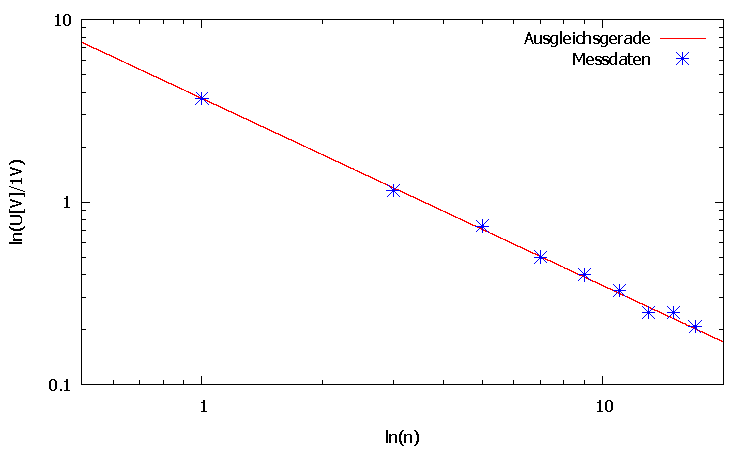
\includegraphics[width = 8cm]{img/rechteck.pdf}
	\caption{Graphische Darstellung der Fourier-Amplituden einer Rechtecksspannung und einem $a \cdot x^b$ fit.}
	\label{gra:recht}

	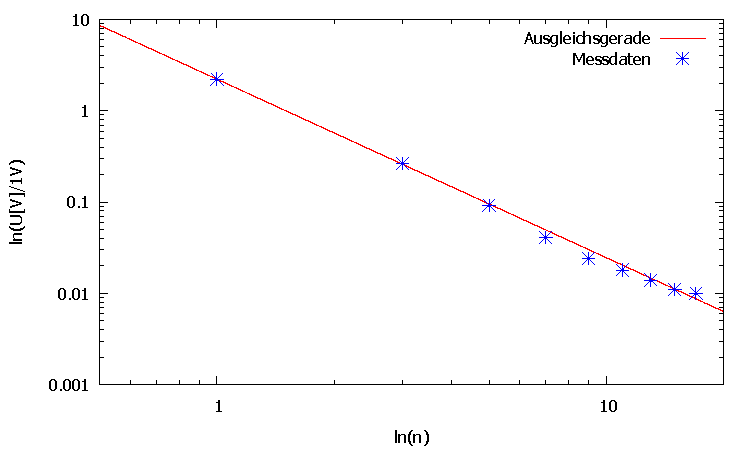
\includegraphics[width = 8cm]{img/dreieck.pdf}
	\caption{Graphische Darstellung der Fourier-Amplituden einer Dreiecksspannung und einem $a \cdot x^b$ fit.}
	\label{gra:dreieck}

	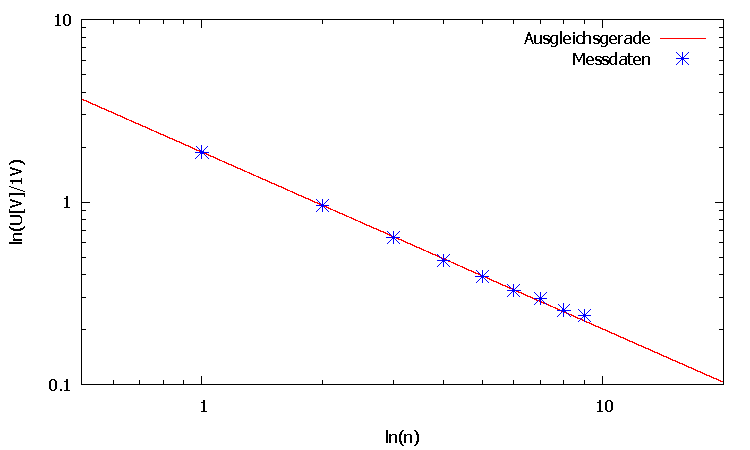
\includegraphics[width = 8cm]{img/saegezahn.pdf}
	\caption{Graphische Darstellung der Fourier-Amplituden einer S"agezahnspannung und einem $a \cdot x^b$ fit.}
	\label{gra:saege}
\end{figure}

\clearpage


\begin{table}[!h]
\begin{center}
\begin{tabular}{|r|r|r|r|r|r|}
\hline
 Rechteck & & Saegezahn & & Dreieck & \\
 n-te Oberwelle & U[V] & n-te Oberwelle & U[V] & n-te Oberwelle & U[V] \\
\hline
\hline
1	& 3.700 & 1	& 1.880 & 1	& 2.220 \\
3	& 1.160 & 2	& 0.960 & 3	& 0.266 \\
5	& 0.740 & 3	& 0.640 & 5	& 0.092 \\
7	& 0.500 & 4	& 0.480 & 7	& 0.041 \\
9	& 0.400 & 5	& 0.392 & 9	& 0.024 \\
11	& 0.328 & 6	& 0.328 & 11& 0.018 \\
13	& 0.248 & 7	& 0.296 & 13& 0.014 \\
15	& 0.249 & 8	& 0.256 & 15& 0.011 \\
17	& 0.208 & 9	& 0.240 & 17& 0.010 \\
\hline
\end{tabular}
\caption[]{Messwerte der Spannung $U$ bei der n-ten Oberschwingung}
\label{tab:messwerte}
\end{center}
\end{table}


Bei der Messung der ersten 9, von null verschiedenen, Fourieramplituden einer Rechtecks-, einer Dreiecks- und einer S"agezahnschwingung ergaben sich die in Tabelle \ref{tab:messwerte} gemessenen Werte. Die Daten sind in den Graphiken \ref{gra:recht}, \ref{gra:dreieck} und \ref{gra:saege} dargestellt.

Eine Ausgleichsrechnung mithilfe der Funktion $a*x^b$ ergab folgende Werte:

\begin{eqnarray*}
	&\text{Dreiecksspannung}& \\
	a &=& \SI{2.220 (5)}{} \\
	b &=& \SI{-1.955 (14)}{} \\
	&\text{Rechtecksspannung}& \\
	a &=& \SI{3.695  (22)}{} \\
	b &=& \SI{-1.025 (9)}{} \\
	&\text{S"agezahnspannung}& \\
	a &=& \SI{1.878 (9)}{} \\
	b &=& \SI{-0.968 (7)}{}
\end{eqnarray*}


Bei der Rechtecks- und S"agezahnspannung ist eine erwartete Abnahme der Amplitude mit 1/x erkennbar.
Die Dreiecksspannung hingegen l"asst eine erwartete 1/$x^2$ Abh"angigkeit erkennen.

Die geringen Abweichungen des Exponenten von den Erwarteten k"onnten sich durch die Analyse Bauteile des Oszilloskops erkl"aren lassen. 

\clearpage

\subsection{Sukzessive Zusammensetzung verschiedener Schwingungsformen aus deren Komponenten}
\label{sub:sukzessive_zusammensetzung_verschiedener_schwingungsformen_aus_deren_komponenten}

\begin{figure}[!h]
	\centering
	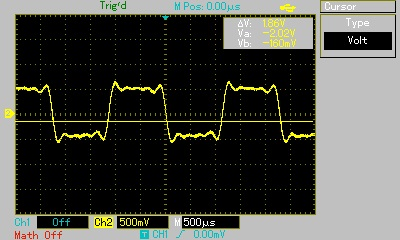
\includegraphics[width = 8cm]{img/rechteck.jpg}
	\caption{Fouriersynthese einer Rechtecksspannung aus den ersten 9 Oberschwingungen.}
	\label{fg:recht}

	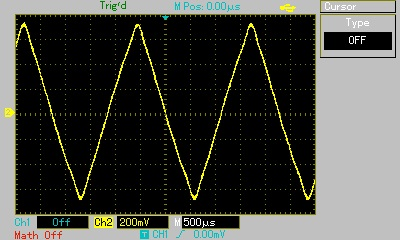
\includegraphics[width = 8cm]{img/dreieck.jpg}
	\caption{Fouriersynthese einer Dreiecksspannung aus den ersten 9 Oberschwingungen.}
	\label{fg:dreieck}

	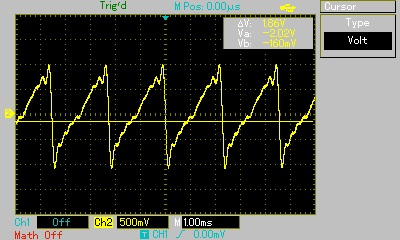
\includegraphics[width = 8cm]{img/saege.jpg}
	\caption{Fouriersynthese einer S"agezahnspannung aus den ersten 9 Oberschwingungen.}
	\label{fg:saege}
\end{figure}
\clearpage

\begin{table}[!h]
\begin{center}
\begin{tabular}{|r|r|r|r|r|r|}
\hline
Rechteck & & Dreieck & & S"agezahn & \\
n-te Oberschwingugn & U[V] & n-te Oberschwingugn & U[V] & n-te Oberschwingugn & U[V]\\
\hline
\hline
1 & 0.600 & 1 & 0.600 & 1 & 0.600\\
2 & 0.000 & 2 & 0.000 & 2 & -0.300\\
3 & 0.200 & 3 & 0.067 & 3 & 0.200\\
4 & 0.000 & 4 & 0.000 & 4 & -0.150\\
5 & 0.120 & 5 & 0.024 & 5 & 0.120\\
6 & 0.000 & 6 & 0.000 & 6 & -0.100\\
7 & 0.085 & 7 & 0.012 & 7 & 0.085\\
8 & 0.000 & 8 & 0.000 & 8 & -0.075\\
9 & 0.065 & 9 & 0.007 & 9 & 0.065\\
\hline
\end{tabular}
\caption[]{Werte der theoretisch errechneten Amplituden aus den Fourier-Koeffizienten.}
\label{tab:amplituden}
\end{center}
\end{table}

Bei der sukzessiven Zusammensetzung verschiedener Schwingungsformen aus deren Komponten ergaben sich f"ur die Rechtecksspannung, die Dreiecksspannung und die S"agezahnspannung die in den Graphiken \ref{fg:recht}, \ref{fg:dreieck} und \ref{fg:saege} gezeigten Bilder auf dem Oszilloskop.

F"ur die Oberschwingungen wurden die in Tabelle \ref{tab:amplituden} aufgef"uhrten Werte verwendet, welche zuvor aus den Fourierkoeffizienten errechnet wurden.